\documentclass[crop,tikz]{standalone}% 'crop' is the default for v1.0, before it was 'preview'
%\usetikzlibrary{...}% tikz package already loaded by 'tikz' option
\usetikzlibrary{arrows.meta,calc,decorations.markings,math,arrows.meta}


\definecolor{prevcol}{RGB}{43,131,186}
\definecolor{artcol}{RGB}{253,174,97}
\definecolor{mortcol}{RGB}{215,25,28}
\definecolor{popcol}{RGB}{171,221,164}
\definecolor{pdrcol}{RGB}{160,32,240}

\begin{document}
	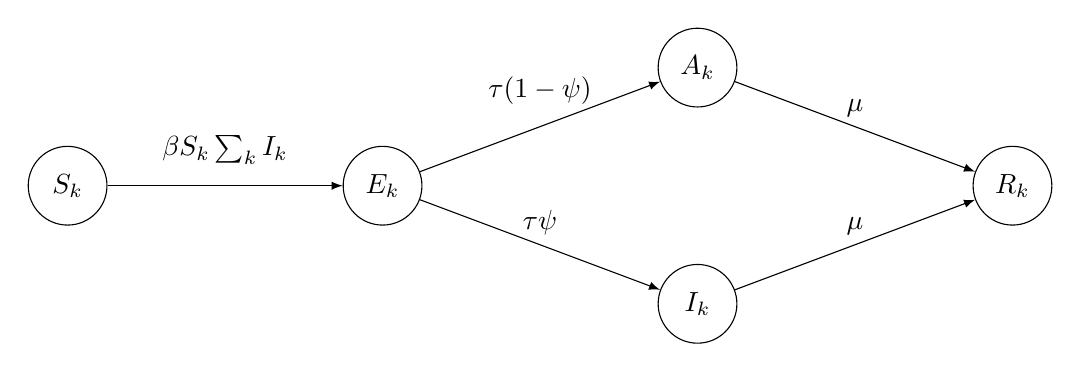
\begin{tikzpicture}
% cascade of care
\node[circle, draw, inner sep=0pt, minimum size=1cm] (S) at (0,0) {$S_k$};
\node[circle, draw, inner sep=0pt, minimum size=1cm] (E) at (4,0) {$E_k$};
\node[circle, draw, inner sep=0pt, minimum size=1cm] (I) at (8,-1.5) {$I_k$};
\node[circle, draw, inner sep=0pt, minimum size=1cm] (A) at (8,1.5) {$A_k$};
\node[circle, draw, inner sep=0pt, minimum size=1cm] (R) at (12,0) {$R_k$};
%\node[circle, draw, inner sep=0pt, minimum size=1cm,dashed] (C) at (8,-3) {$C_k$};

\draw[->,>=latex] (S) edge node[yshift=13pt] { $\beta S_k \sum_k I_k$} (E);
%\draw[->,>=latex] (E) edge[bend left=16] node[yshift=-13pt] {  } (C);
\draw[->,>=latex] (E) edge node[above] { $\tau\psi$ } (I);
\draw[->,>=latex] (E) edge node[yshift=13pt] { $\tau(1-\psi)$ } (A);
\draw[->,>=latex] (A) edge node[above] { $\mu$ } (R);
\draw[->,>=latex] (I) edge node[above] { $\mu$ } (R);

%
%\node[inner sep=0pt, minimum size=1cm,anchor=west] (C2) at (9.5,-2.3) {{\small Reported cases in age group $k$ on day $t$}:};
%\node[inner sep=0pt, minimum size=1cm,anchor=west] (C3) at (9.9,-2.7) {{\small  $J_k(t)=\rho_k\left[C_k(t)-C_k(t-1)\right]$}};
%
%
%\node[inner sep=0pt, minimum size=1cm,anchor=west] (D2) at (9.5,-3.7) {{\small Reported deaths in age group $k$ on day $t$}:};
%\node[inner sep=0pt, minimum size=1cm,anchor=west] (D3) at (9.9,-4.1) {{\small  $D_k(t)= \epsilon_k\sum_d \left[ J_k(t-d)\gamma_d \right]  $}};
%
%\draw[->,>=latex,dashed] (C) -- (C2.west);
%\draw[->,>=latex,dashed] (C) -- (D2.west);


\end{tikzpicture}
\end{document}